\documentclass[10pt]{article}
\usepackage[margin=0.7in]{geometry}
\usepackage{graphicx,mathptmx}
\usepackage[hidelinks]{hyperref}
\title{Native finite-size extensions: implementation receipt}
\author{Bounded development correctness; no performance claim}
\date{30 October 2026}
\begin{document}
\maketitle
\noindent The user requested implementation of review items 1--5. These add
opt-in selector, exact-contraction, partial-relation and binary/orbit paths.
The original solver, seeded defaults, certificate replay and source packet
guards remain available. No scientific experiment or benchmark ran.
\begin{center}
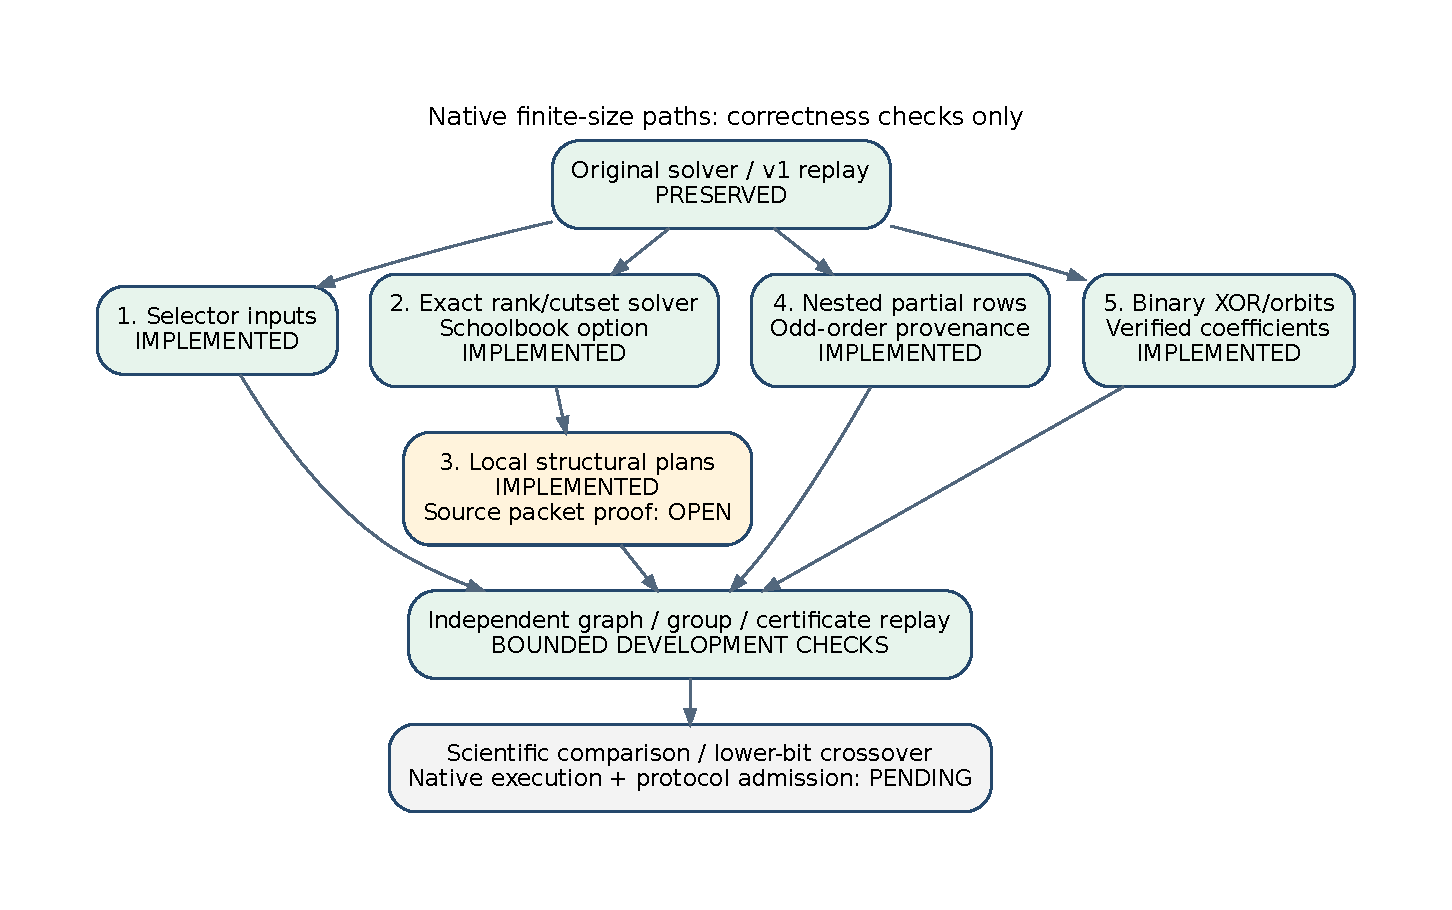
\includegraphics[width=\linewidth,height=3.0in,keepaspectratio]{implementation.pdf}
\end{center}
\noindent\textbf{1. Selector inputs: implemented and development-checked.}
The engine branches on inverse-hash interval values, caches bounded decodes,
retains slot identities and optionally derives the final point from the sum
equation. A separate tensor encoder makes selectors the actual free inputs.
All returned points pass independent subgroup, hash and sum replay. Decoder
randomness is separate from the label RNG. The alternative graph counts
decoded tuples, not cofactor-projection preimages. Generic tuple search and
decoder work remain; no exponent improvement is established.

\medskip\noindent\textbf{2. Encoding and solver choice: implemented and checked.}
A greedy rank planner and exact BigUint variable elimination admit low-rank
tables and exhaustive cutset children under explicit resource policies.
Witness-only search propagates exact local support without requesting count
precision and checks the full graph before returning. A schoolbook/ripple
product is an optional alternative to the unchanged Fourier default. Opaque
predicates are not assumed cheaply factorable. No optimal-width guarantee,
SAT/CNF-XOR exporter, approximate-zero fallback or performance result is claimed.

\medskip\noindent\textbf{3. Checked local plans: partial against the proposal.}
Admission recomputes the graph/pin edge partition and all intermediate ranks;
execution checks live storage and covers all cutset assignments. This is
finite exact conditioning, not a new small-parameter Appendix D packet
schedule. Smaller-packet packing, coefficient coverage, precision,
reconstruction, shrinkage and cost obligations remain open. The original
massive packet-recursion onset is unchanged. No new theorem or Lean proof
is claimed, and bounded controls do not replace the independent audit.

\medskip\noindent\textbf{4. Partial relations: implemented and checked.}
Nested bases require the same prime/hash seed with ordered thresholds.
The bounded collector admits up to two outer points, pivots outer columns
before inner columns, and retains every original labelled row and its
provenance. Arithmetic is modulo the odd subgroup prime, not XOR cycle
cancellation. Independent replay checks memberships, group equations,
all column cancellations and scalar extraction. A known r=7 control uses
coefficient 6 rather than binary coefficient 1. A separate bounded query
driver generates uniform labels without exposing them to the witness solver.

\medskip\noindent\textbf{5. Binary specialization: implemented components.}
Native polynomial arithmetic verifies irreducibility and inverses. The
odd-degree Koblitz constructor checks primality proofs, generator and full
cardinality by Hasse uniqueness or exact bounded counting. Half-trace
decompression is canonical. Full-rank affine XOR hashes have checked inverse
fibers. Frobenius eigenvalue candidates come from the known Koblitz polynomial
and are checked on the generator; representative coefficients receive scalar
replay. Orbit domains expand all selected orbits, including shorter ones.
Changed hash distributions need their own coverage analysis. This does not
establish full official binary setup, a challenge solve or a prime-field
specialization.

\section*{Validation scope, identities and remaining work}
\noindent The known-answer prime fixture is p=5, a=2, b=1, r=7, h=1,
G=(0,1); library target [3]G=(3,3), existing CLI target [4]G=(3,2).
A second fixture has p=5, a=0, b=1, r=3, h=2, G=(0,1).
Binary fixtures use f=x$^5$+x$^2$+1, r=11 and
y$^2$+xy=x$^3$+ax$^2$+1: a=0, h=4, G=(4,22), Frobenius eigenvalue 4;
a=1, h=2, G=(10,18), eigenvalue 5. The official degree-131 polynomial
x$^{131}$+x$^{13}$+x$^2$+x+1 passes irreducibility checking; that is field-only
validation. Complete official order/generator/target validation is not claimed.

\medskip\noindent Controls compare exhaustive small domains/targets and graph
truth tables, pins and conditioned counts; forged witnesses/plans, invalid
codes, singular hashes, isolated false predicates and resource exhaustion;
full known-answer IC and partial recovery; original CLI replay and exclusive
creation; independent small carryless products, group/cardinality/Frobenius
identities, complete orbit enumeration and coefficient replay. A 70-edge
witness succeeds under a one-bit precision policy while exact counting is
correctly refused. The source-compatible default certificate controls stay
in the full suites. Raw final transcripts, source manifests and exact commands
are in README.md and VALIDATION.md. Local test durations are not benchmarks.

\medskip\noindent The parent report retains primary sources and negative
SAT/enumeration evidence. Sources include
\href{https://github.com/bochum-crypto/subexponential-ecdl/tree/1ee44e562b1b9a50ea339f3b8f81112b5a24b96f}{Bochum v0.2},
\href{https://arxiv.org/abs/1908.04381}{TensorOrder},
\href{https://pmc.ncbi.nlm.nih.gov/articles/PMC7334981/}{WDSat}, and
\href{https://github.com/isogeny-labs/crypto-autoresearcher/tree/fc26d24369e56ad20995380475989c40a5e0e84f/knowledge/leads/ecdlp}{the pinned lead atlas}.
No comprehensive novelty or independent mathematical audit is completed.

\medskip\noindent The original frozen A/B panel and both challenge scalars
remain unresolved. Earlier S3 upload/readback succeeded; authenticated native
image/execution and measurement admission remain unverified. The measurement
card stays draft pending its driver, exact protocol/identities, checker,
cost envelope and execution-host checkpoint. No chat credentials were reused.
No performance, scaling or sub-rho conclusion follows from this receipt.
Canonical graphs receive no measured value or curve-transport edge.
\end{document}
